\documentclass{sig}

\usepackage{algorithm}
\usepackage{algpseudocode}
\usepackage{amsmath}
\usepackage{appendix}
\usepackage{balance}
\usepackage{caption}
\usepackage{color}
\usepackage{comment}
\usepackage{epstopdf}
\usepackage{graphicx}
\usepackage{listings}
\usepackage{mathtools}
\usepackage{microtype}
\usepackage{multirow}
\usepackage{pdfpages}
\usepackage{subcaption}
\usepackage{subfig}
\usepackage{tabularx}
\usepackage{times}
\usepackage{url}
\usepackage{xcolor}
\usepackage{xspace}
\usepackage{bm}
\usepackage{mdwlist}

\newcommand{\subparagraph}{}
\usepackage{titlesec}

\titlespacing{\section}{0ex}{0.8ex}{0ex}
\titlespacing{\subsection}{0ex}{0.8ex}{0ex}
\titlespacing{\subsubsection}{0ex}{0.7ex}{0ex}
\setlength{\parskip}{0ex}

\algrenewcommand\alglinenumber[1]{\scriptsize #1:}

\makeatletter
\renewcommand*{\ALG@name}{Investing Rule}
\makeatother


\usepackage{breqn}
\interfootnotelinepenalty=10000

\newcommand{\todo}[1]{\textcolor{blue}{TODO: #1}}
\newcommand{\done}[1]{\textcolor{green}{DONE#1}}
\newcommand{\tim}[1]{\textcolor{red}{Tim: #1}}
\newcommand{\lore}[1]{\textcolor{blue}{Lorenzo: #1}}
\newcommand{\ez}[1]{\textcolor{orange}{ez: #1}}
\newcommand{\sam}[1]{\textcolor{purple}{sam: #1}}
\newcommand{\carsten}[1]{\textcolor{brown}{Carsten: #1}}

\newcommand{\naive}{na\"{\i}ve\xspace}
\newcommand{\Naive}{Na\"{\i}ve\xspace}
\newcommand{\naively}{na\"{\i}vely\xspace}

\newcommand{\ainv}{$\alpha$-investing }
\newcommand{\sfdr}{Sequential-FDR }
\newcommand{\mfdre}{$mFDR_{\eta}$ }
\newcommand{\mfdr}[1]{$mFDR_{#1}$}
\newcommand{\Ex}[1]{E\left[#1\right]}
\newcommand{\Prob}[1]{\text{P}\left(#1\right)}
\newcommand{\CProb}[2]{\text{P}\left(#1|#2\right)}
\newcommand{\pval}{$p$-value }
\newcommand{\pvals}{$p$-values }


\newcommand{\system}{{\sc Aware}}
\newcommand{\Chi}{\mathcal{X}}

\newtheorem{theorem}{Theorem}
\newtheorem{lemma}{Lemma}


%\setlength\abovedisplayskip{0pt plus 2pt minus 0pt}
%\setlength\belowdisplayskip{0pt plus 2pt minus 0pt}

%\makeatletter
%\g@addto@macro \normalsize {%
%\setlength\abovedisplayskip{0pt plus 2pt minus 0pt}%
%\setlength\belowdisplayskip{0pt plus 2pt minus 0pt}%
%\setlength\abovedisplayshortskip{0pt plus 2pt minus 0pt}%
%\setlength\belowdisplayshortskip{0pt plus 2pt minus 0pt}%
%}
%\makeatother

%\makeatletter
%\g@addto@macro \small {%
%\setlength\abovedisplayskip{0pt plus 2pt minus 0pt}%
%\setlength\belowdisplayskip{2pt plus 2pt minus 0pt}%
%\setlength\abovedisplayshortskip{0pt plus 2pt minus 0pt}%
%\setlength\belowdisplayshortskip{2pt plus 2pt minus 0pt}%
%}
%\makeatother

\DeclareMathOperator*{\argmin}{\arg \min}
\DeclarePairedDelimiter\ceil{\lceil}{\rceil}

\captionsetup{font={bf}}

%\newcommand{\system}{{\sc Vizdom}}

\newcommand{\specialcell}[2][c]{
  \begin{tabular}[#1]{@{}c@{}}#2\end{tabular}}

\definecolor{dark-gray}{gray}{0.2}

\newenvironment{packed_item}{
\begin{list}{$\bullet$}{
  \setlength{\itemsep}{-2pt}
  \setlength{\parskip}{1pt}
  \setlength{\labelwidth}{15 pt}
  \setlength{\leftmargin}{10pt}
  \setlength{\itemindent}{0pt}}
}{\end{list}}

% for floated 2 column equations
\newcounter{tempEquationCounter}
\newcounter{thisEquationNumber}
\newenvironment{floatEq}
{\setcounter{thisEquationNumber}{\value{equation}}\addtocounter{equation}{1}% record equation as happened and remember number
\begin{figure*}[t]% float following equation across columns
\normalsize\setcounter{tempEquationCounter}{\value{equation}}% record current equation number in floated location
\setcounter{equation}{\value{thisEquationNumber}}% use previous equation number
}
{\setcounter{equation}{\value{tempEquationCounter}}% set back to equation number in floated location
\hrulefill\vspace*{4pt}% add a horizontal rule separator
\end{figure*}% end float environment
}
\newtheorem{defi}{Definition}
\makeatletter
\newenvironment{subheuristic}[1]{%
  \def\subtheoremcounter{#1}%
  \refstepcounter{#1}%
  \protected@edef\theparentnumber{\csname the#1\endcsname}%
  \setcounter{parentnumber}{\value{#1}}%
  \setcounter{#1}{0}%
  \expandafter\def\csname the#1\endcsname{\theparentnumber\alph{#1}}%
  \ignorespaces
}{%
  \setcounter{\subtheoremcounter}{\value{parentnumber}}%
  \ignorespacesafterend
}
\makeatother
\newcounter{parentnumber}

\newtheorem{heuristic}{Heuristic}

\begin{document}



\title{An Interactive Data Exploration Tool that Controls False Discoveries}

\numberofauthors{1}
\author{
\alignauthor
\vspace*{-30pt}
%Paper \#178
\begin{tabular}{cccc}
\end{tabular}\\
\vspace{1.5mm}
\affaddr{Department of Computer Science, Brown University}\\
\vspace{0.75mm}
\{firstname\_lastname\}@brown.edu
%\email{\{firstname\_lastname\}@brown.edu}
}

%\numberofauthors{6}
%\author{
%\small{Andrew Crotty, Alex Galakatos, Kayhan Dursun, Tim Kraska, Ugur Cetintemel, Stan Zdonik} \\
%\small{Department of Computer Science, Brown University} \\
%\small{\{crottyan, agg, kayhan, kraskat, ugur, sbz\}@cs.brown.edu}
%}
\date{}
\maketitle

\begin{abstract}

\end{abstract}



\section{Introduction}
\label{sec:intro}
In the era of Big Data, interactive data exploration tools arise as an important mean to explore and derive insights from data through visualization.  
However, perceived interesting patterns in visual data representations, such as relationships or trends, may emerge from irrelevant random effects inherent to the data, such as random noises, large variances, insufficient samples, and biases. 
Without proper statistical control, users may mistake a distinct or dominant visual observation as statistically significant.  
On the other hand, systems that search and recommend visualizations automatically based on such interesting visual features further increase the chance of bogus insights.  
A recent study highlights these issues and shows that visualization and recommendation systems that do not consider the risk of false discovery, such as Vizdom~\cite{vizdom}, SeeDB~\cite{seedb} and Data Polygamy~\cite{polygamy}, become difficult to derive insights safely on real-world datasets \cite{binnig2017sustainable}.

False discovery due to random noise is pervasive in visual data exploration on real-world datasets. For example, when using Vizdom~\cite{vizdom} to explore a recently conducted survey on personal habits and opinions~\cite{binnig2017sustainable}, we observed that the preference on watching films on DVD produced visually different proportions of belief in aliens, as shown in Figure~\ref{fig:example} (A and B).
Just by visually examining these charts, users often falsely assumed that people who prefer to watch movies on DVD are more prone to believe in aliens even though this effect is not statistically significant.
%But such predictor proved neither much sensible nor statistically significant.  

Such observation-based hypotheses may be accumulated quickly as the user continues to explore a dataset, and hence dramatically raises the risk of spurious findings. 
With the same survey dataset, after searching through a few different comparisons we stumbled upon a visualization that suggests hair color predicts whether one knows about Michael Stonebraker, and it would be statistically significant if considered as a lone hypothesis. This phenomenon is often referred to as data dredging or $p$-hacking~\cite{head2015extent}, and formally known as the multiple comparison problem~\cite{shaffer1995multiple}.

Several challenges exist to control false insights in such interactive data exploration.  
The first question is what could even be considered as a hypothesis in visual data exploration.
In some cases users might explicitly specify certain hypotheses, but in other instances they do not formulate any hypothesis but still use visualization to infer about the data or to extract an insight.
An ideal system should assist users in hypothesis formulation and corresponding hypothesis test selection.

Second, interactive data exploration mandates that hypotheses are formulated dynamically based on the process of human decision making.  
However the classical statistical procedures such as Bonferroni~\cite{bonferroni1936teoria} and Sequential FDR~\cite{g2016sequential} are not dynamic as they require collecting all the hypotheses a priori before finalizing any significance result.  
Moreover these traditional techniques assume complete pass of the dataset, and thus would make the system non-interactive on larger data.  
Thus an ideal system for interactive control of false discovery should follow progressive computation, which proves to be a more appealing paradigm~\cite{vizdom, onlineagg, zgraggen2016progressive}.  

Finally, parts of the data exploration process can be automated through algorithmic search and recommendation. Such automatic data exploration should also be subject to false discovery control.  

In this demo, we present \system{}\footnote{\system{} stands for Quantifying the Uncertainty in Data Exploration.}, a first ``safe'' visual data exploration tool that addresses these challenges. 
In \system{}, we implemented recent techniques in interactive false discovery control that are both dynamic and progressive~\cite{zhao2016controlling}, apply them to visual data exploration and visualization recommendation, and expose them through a pen- \& touch-based user interface that simplifies and in some cases even automates the creation of hypothesis tests.


%Thus, to address theses challenges, we implemented the recent advance in interactive false discovery control that is both dynamic and progressive, and applied to both visual data exploration and recommendation~\cite{zhao2016controlling}. 

\begin{figure}
\centering
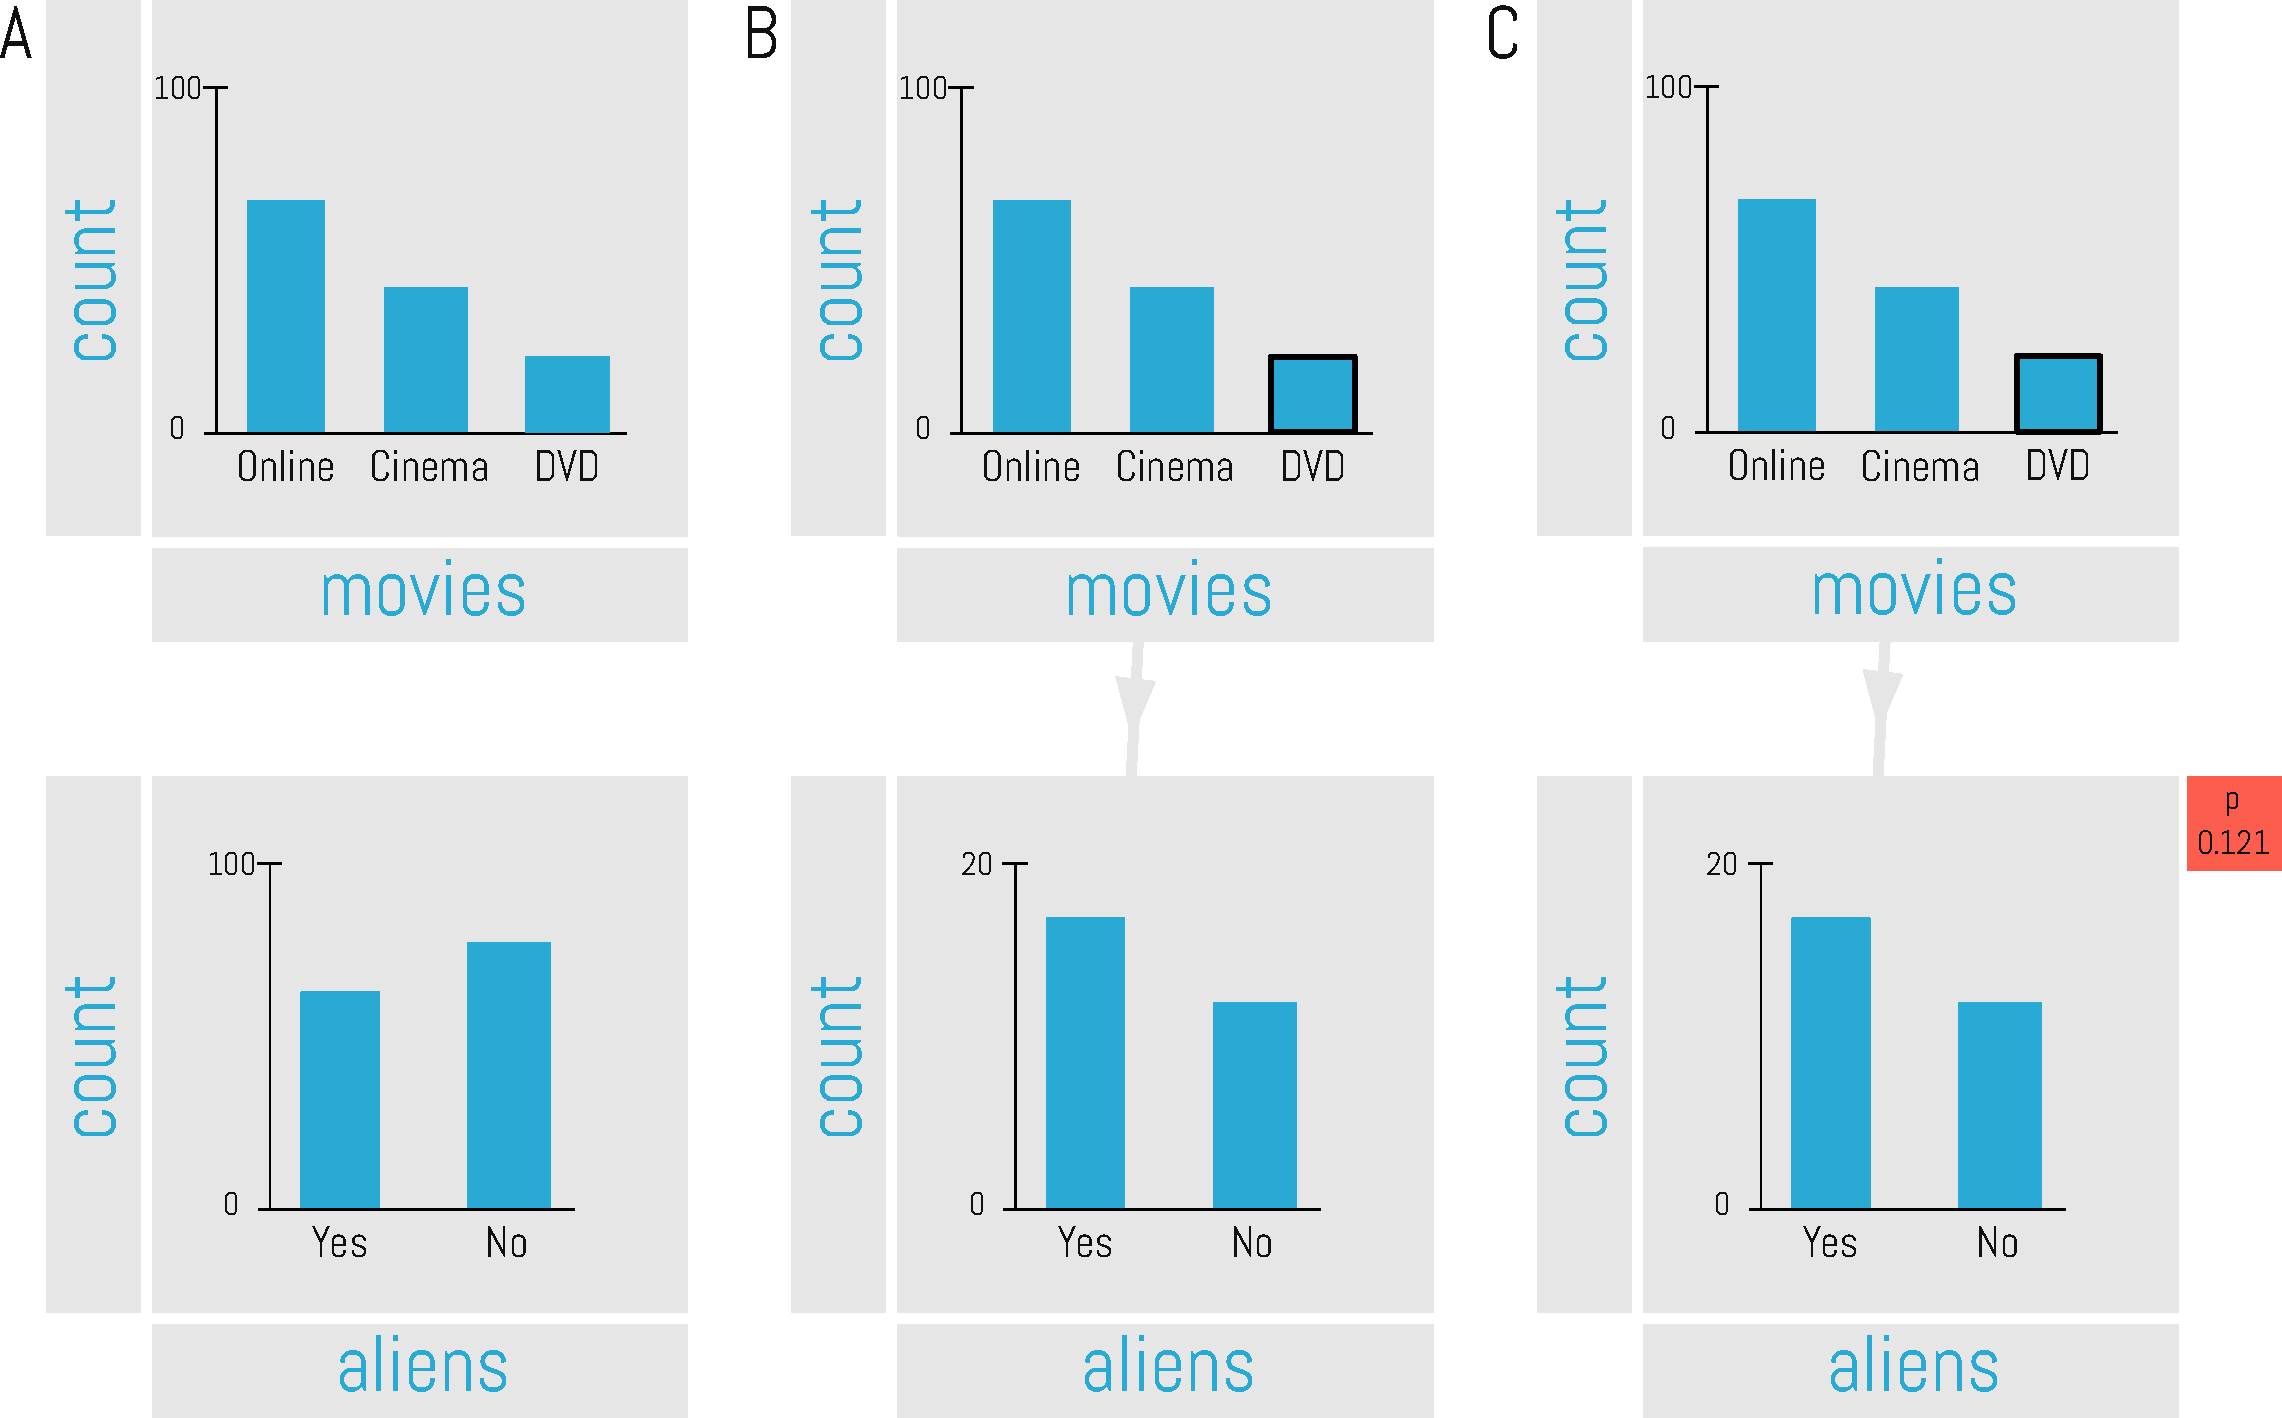
\includegraphics[width=0.47\textwidth]{figures/example}
\caption{Example of a visualization network where users might be led to false discoveries without automatic hypothesis formulation. (A) two separate visualizations showing preferences for watching movies and how many people believe in alien existence; (B) the two visualizations combined where the bottom one shows proportions of belief in alien existence for only people who like to watch movies on DVD, displaying a noticeable difference compared to the overall population. (C) same visualizations as before but now with automatic hypothesis formulation turned on, highlighting that the observed effect is not statistically significant.}
\label{fig:example}
\vspace{-3.5ex}
\end{figure}

%\begin{figure*}[ht]
\begin{center}
  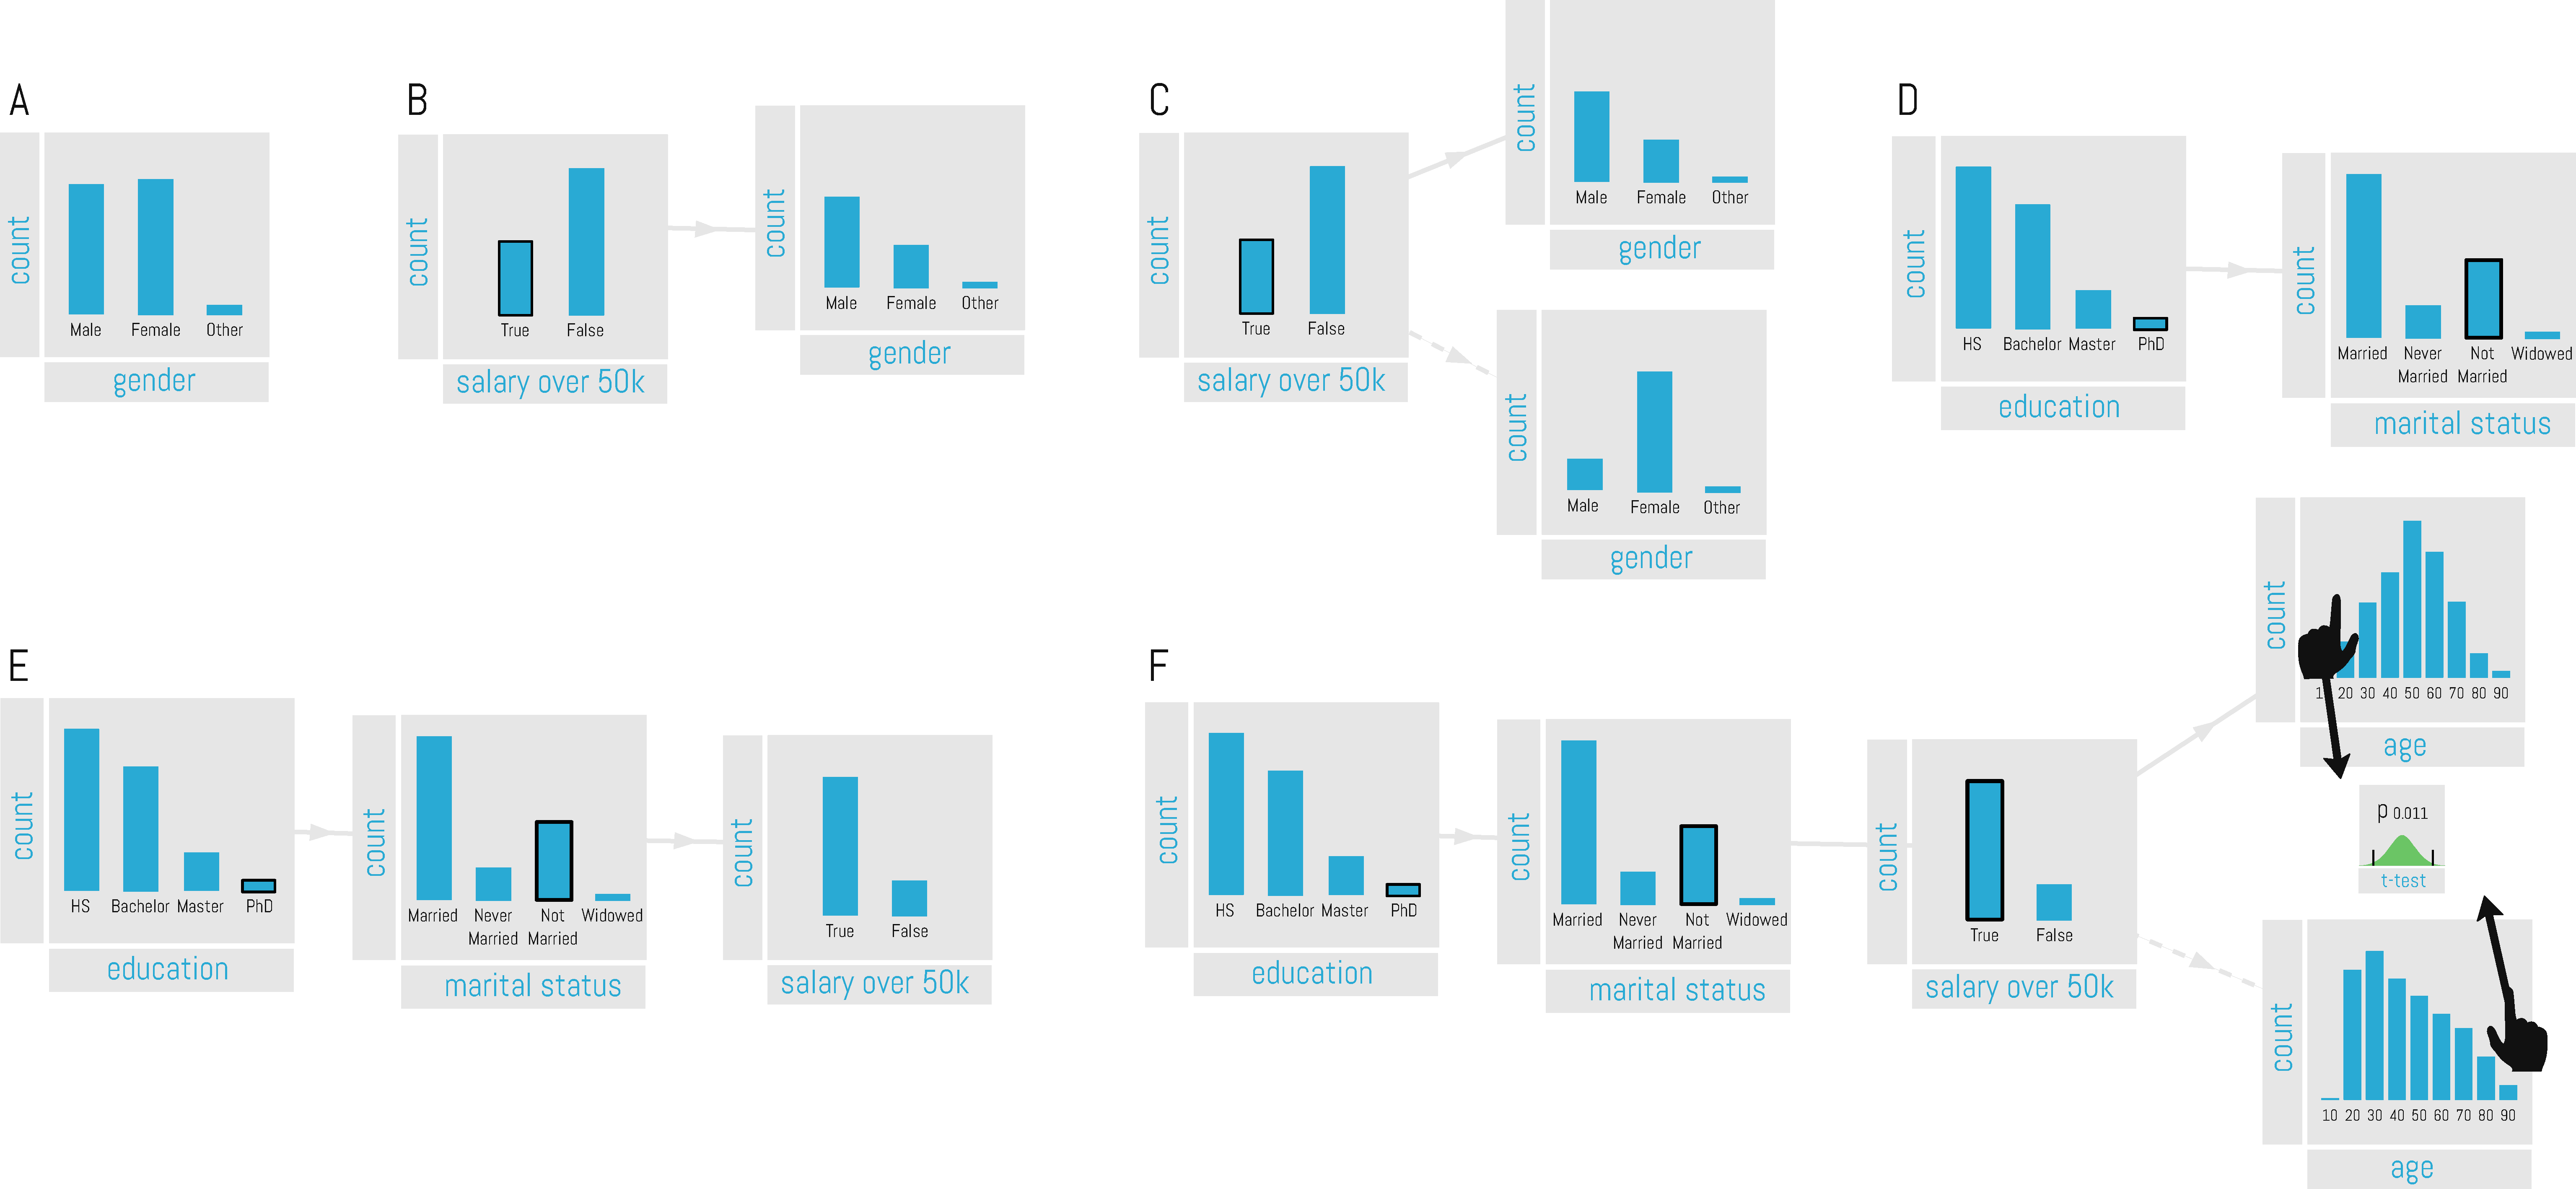
\includegraphics[width=0.9\textwidth]{figures/storyboard}
\end{center}\vspace{-5.5ex}
\vspace{-2.5ex}
\caption{An example Interactive Data Exploration Session}
\vspace{-3.5ex}
\label{fig:sb}	
\end{figure*}

\subsection{Visualizations as Hypotheses}
A visualization per-se shows a descriptive statistic (e.g., the count of women or the count of men) of the dataset and is not a hypothesis. 
It is reasonable to assume that in step~A of Figure~\ref{fig:sb} the user just looks at the gender distribution and simply acknowledges that the census surveys roughly the same amount of women and men.
However, it becomes an hypothesis test, if the user expected something else and draws a conclusion/inference based on the visualization. 
For example, if the user somehow assumed that there should be more men than women in the data and therefore considering the fact that there is an equal amount as an insight.
The notion of a visualization being considered as a hypothesis becomes even clearer in step~(B) and (C) of the example work-flow.
When looking at the visualization in (B) in isolation, it just depicts a descriptive statistic. 
Indeed, if the user would just take it as such and not make any inference about it and/or base further exploration on an insight extracted from this visualisation, then it would not be considered an hypothesis.
We argue however that the opposite is true more often than not. First, our analytical reasoning and sense-making process is inherently non-linear \cite{pirolli2005sensemaking,shrinivasan2008supporting}.
Our future actions are influenced by new knowledge we discovered in previous observations.
Second, while susceptible to certain types of biases \cite{attractionBias}, the human visual system is highly optimized at picking up differences in visual signals and at detecting patterns \cite{burgess1981efficiency}. 
An average user is very likely drawn to the changes between the gender distribution of step (A) and step (B) and might therefore infer that women earn less than men and potentially flag this as an interesting insight that deserves more investigation.
This is illustrated in step~(C) where the user now further drills down and visually compares the distribution of gender filtered by salary. 
We qualitatively confirmed this notion through a formative user study where we manually coded user-reported insights, following a think-aloud protocol similar to the one proposed in ~\cite{guo2016case}. In this study we observed that users tend to pick up on even slight differences in visualizations and regard them as insights and users predominantly base future exploration paths on previously inferred insights. 

We conclude two things: (1) most of the time users indeed treat visualizations as hypotheses, though there are exceptions, and (2) they often (wrongly) assume that what they see is statistical significant. 
The latter is particularly true if the users do not carefully check the axis on the actual count.  
For example, if a user starts to analyze the outliers of a billion record dataset and makes the conclusion that mainly uneducated whites are causing the outliers, the dataset she is referring to might be comparable small and the chance of randomness might be much higher. 
The same argument also holds against the critic, that with enough data observing differences by chance are much less likely, which is true. 
As part of visual data exploration tools, users often explore sub-populations, and while the original dataset might be large, the sub-population might be small. 
Thus, we argue that every visualization as part of a interactive data exploration tool should be treated as a hypothesis and that users should be informed about the significance of the insights they gain from the visualization. 
At the same time, a user should have the choice to declare a visualization as just descriptive. 

%\ez{i don't know this ref so not sure where to appropriately fit it in. - This effect is not new and lead for example to areas like visual data mining \cite{visualdatamining}}

\subsection{Heuristics for Visualization Hypotheses}
A core question remains: what should the hypothesis for a visualization be. 
Ideally, users would tell the system every single time what they are thinking so that the hypothesis is adjusted based on their assumed insight(s) they gain from the visualization. 
However, this is disruptive to any interactive data exploration session. 
We rather argue that the system should use a good default hypothesis, the user can modify (or even delete) if she so desires. 
For the purpose of this work, we mainly focus on histograms as shown in Figure~\ref{fig:sb} and acknowledge that there exist many other visualizations, which we consider as future work. 
We derived the following heuristics from two separate user studies where we observed over 50 participants using a IDE tool to explore various datasets. 

\vspace{-1.75ex}
\begin{enumerate*}
    \item {\em Every visualization without any filter conditions is not a hypothesis (e.g., step~A in Figure~\ref{fig:sb}) unless the user makes it one. } This is reasonable, as users usually first gain a general high-level impression of the data. Furthermore, in order to make it an hypothesis, the user would need to provide some prior knowledge/expectation, for example as discussed before, that he expected more men than women in the dataset. 
    \item {\em Every visualization with a filter condition is a hypothesis with the null-hypothesis that the filter condition makes no difference compared to the distribution of the whole dataset}. For example, in step~B of Figure~\ref{fig:sb} the null hypothesis for the distribution of men vs. women given the high salary class of over $\$50k$ would be that there is no difference compared to the equal distribution of men vs. women over the entire dataset (the visualization in step~A). This is again a reasonable assumption as the distribution of an attribute given others is only interesting, if it shows some different effect compared to looking at the whole dataset. 
    \item {\em If two visualization with the same but some negated filter conditions are put next to each other, it is a test with the null-hypothesis that there is no difference between the two visualized distributions, which supersedes the previous hypothesis.} This is the case in step~C: given that the user looks explicitly at the distribution of males vs females given a salary over and under $\$50k$ is a strong hint from the user, that he wants to compare these two distributions. 
\end{enumerate*}
\vspace{-2.0ex}

As with every heuristic it is important to note, that the heuristic can be wrong. 
Therefore it is extremely important to allow the user to overwrite the default hypothesis as well as delete default hypothesis if one really just acted as a descriptive statistic or was just generated as part to a bigger hypothesis test. 
Furthermore, there exist of course other potential null-hypothesis.
For example, in our workflow we assume by default that the user aims to compare distributions, which requires a  $\chi^2$-test.
However, maybe in some scenarios comparing the means (i.e., a t-test) might be more appropriate as the default test. Yet, studying in detail what a good default null-hypothesis is dependent on the data properties and domain, is beyond the scope of this paper. 

\subsection{Heuristics Applied to the Example}
For our example in Figure~\ref{fig:sb} the resulting hypothesis could be as follows:
Step~A is not an hypothesis based on rule 1 as it just visualizes the distribution of a single attribute over the whole dataset. 
Step~B is the hypothesis $m_1$ if the distribution of gender is different given a salary over $\$50k$. 
Step~C supersedes the previous hypothesis and replaces it with an hypothesis $m_1'$ if the gender distribution between a salary over and under $\$50k$ is different, which is a sightly different question. 
Step~D creates a hypothesis $m_2$ if the marital status for people with PhDs is different compared to the entire dataset, whereas step-E generates a hypothesis $m_3$ if there is a different salary distribution given not married people with a PhD. 
By studying the age distribution in step~F the system first generated a default hypothesis $m_4$  that the distribution of the ages is different given a PhD and being not married for different salary classes. 
However, the user overwrites immediately the default hypothesis with an hypothesis $m_4'$  about the average age. 
Furthermore, as the previous visualizations in step~D and E might just have been stepping stones towards creating $m_4‘$ the user might or might not delete hypothesis $m_2$ and $m_3$. 
However, if the insights our user gained from viewing the marital status, etc., influenced her to look at the age distribution, she might want to keep them as hypothesis. 

Clearly this is only a very small example, but it already demonstrates the general issues. 
Not every insight the user gains (e.g., the insight that women earn less) is explicitly expressed as a test. 
At the same time, as more the user ``surfs'' around the higher the chance that she finds something which looks interesting, but just appears because of chance. 
In the example above, by the time the user actually performs its first test (step~F), she implicitly already tested at least one other hypothesis and potentially even four others. 
Assuming a targeted \pval of $\alpha = 0.05$, the chance of a false discovery therefore increased to $1 - (1 - \alpha)^2=0.098$ for two hypothesis and up to $1 - (1 - \alpha)^4=0.185$ for four hypothesis. 
While the question of what should count as an hypothesis is highly dependent on the user and can never be fully controlled by any system, we can however, enable the system to make good suggestions and help users to track the risk of making false discoveries by chance. 
Furthermore, this short workflow also demonstrates that hypotheses are built by adding but also by removing attributes. 
As we will discuss later, there exist no good method so far to control the risk of making false discoveries for incremental sessions like the ones created by interactive data exploration systems. 
We therefore develop new methods especially for interactive data exploration in Section~\ref{sec:invest}.
%Finally, the situation gets even worse with automatic visualization recommendation engines or correlation finders, as \cite{cidrrisk} already pointed out. 
%While ``safe'' recommendations are beyond the scope of this paper, we will outline potential initial solutions in Section~\ref{sec:fdrcontrol}.

Finally, it should be noted, that the same problems also exist with exploratory analysis using SQL or other tools. 
However, we argue that the situation is becoming worse by the up-rise of visual exploration tools, like Tableau, which are often used by novice users, who not necessarily reflect enough on their exploration path after they found something interesting. 




%In the following section we outlined the challenges associated with automatic risk control. 
%We therefore describe first a common data exploration session and afterwards derive from it the common challenges. 


%- Incremental
%- Chains
%- Backtracking
%- Select most important hypothesis 
%- Default Hypothesis
%- sustainable recommendations. 

%Say something about old SQL

\section{User Interface}
\label{sec:ui}

As argued in the previous section, user feedback is essential in determining, tracking and controlling the right hypothesis during the data exploration process.
With \system~we created a system that applies our heuristic automatically to all visualizations. We designed \system~'s user interface with a few goals in mind.

First, the user should be able to see the hypotheses the system assumed so far, their \pvals, effect sizes and if they are considered significant and should be able to change, add or delete hypotheses at any given stage of the exploration. 

Second, hypotheses rejection decisions should never change based on future user actions unless the user explicitly asks for it. We therefore require an incremental procedure to control the multiple hypothesis risk that does not change its rejection decisions even if more hypothesis tests are executed.
For example, the system should not state that their is a significant age difference for not married highly educated people, and then later on revoke its assessment just because the user did more tests. 
More formally, if the system determined which hypotheses $m_1 ...  m_n$ are significant (i.e., it rejects the null) or not and the user changes the last hypothesis or adds an hypothesis $m_{n+1}$, which should be the most common cases, the significance of hypotheses $m_1..m_{n}$ should not change. 
However, if the user might change, delete, or add hypothesis $k \in {1,..,n}$, depending on the used procedure we might allow that the significance of hypotheses $m_{k+1}$ to $m_n$ might have to change as well.
%Furthermore, the system automatically reports on the {\bf effect size} as a color coded value based on Cohen's suggestions \cite{something}.
%This is according to best practice, as the effect size (e.g., the age difference) determines how big the observed difference is compared to the variance. 

Third, individual hypothesis descriptions should be augmented with information about how much data $n^{H1}$ the user has to add, under the assumption that the new data will follow the current observed distribution of the data, to make an hypothesis significant. 
While sounding counter-intuitive, as one might (wrongly) imply, it is possible to make any hypothesis true by adding more data, calculating this value is in some fields already common practice. 
For example, in genetics scientist often search (automatically) for correlations between genes and high-level effects (like cancer). 
If such a correlation is found, often because of the multiple hypothesis error the chance of a true discovery is tiny (i.e., the \pval is too high). 
In that case the scientist works backwards and estimates how much more genes she has to to sequence in order to make the hypothesis relevant, expecting that the new data (e.g., gene sequences) follow the same distribution of the data the scientist already has.
However, if the effect was just produced by chance, the new data will be more similar to the distribution of the null-hypothesis and the null will not be rejected.  
%Similar, it is possible for a rejected null-hypothesis to calculate how much data $n^{H0}$ has to be added if the null-hypothesis is true, until the null-hypothesis will be accepted. 
% Eli: This has no statistical meaning.
The required value is generally easy to calculate or approximate,  and are highly valuable for the end-user. 
A small value for $n^{H1}$ in relation to the number of totally tested hypotheses might be an indication that the power (i.e., the chance to accept a true alternative hypothesis) of the test was not sufficiently large. 

And finally, users should be able to bookmark important hypotheses. 
Our system uses default hypothesis throughout the exploration and the user might find it too cumbersome to correct everyone for his real intentions, there might be more hypotheses generated than the user intended to test. 
Even if all hypotheses are what the user was considering, some of them might be more important to her than others; the hypotheses the user would like to include in a presentation or show to her boss. 
A key key question becomes, what is the expected number of false discoveries among those important discoveries?

\begin{figure}
\centering
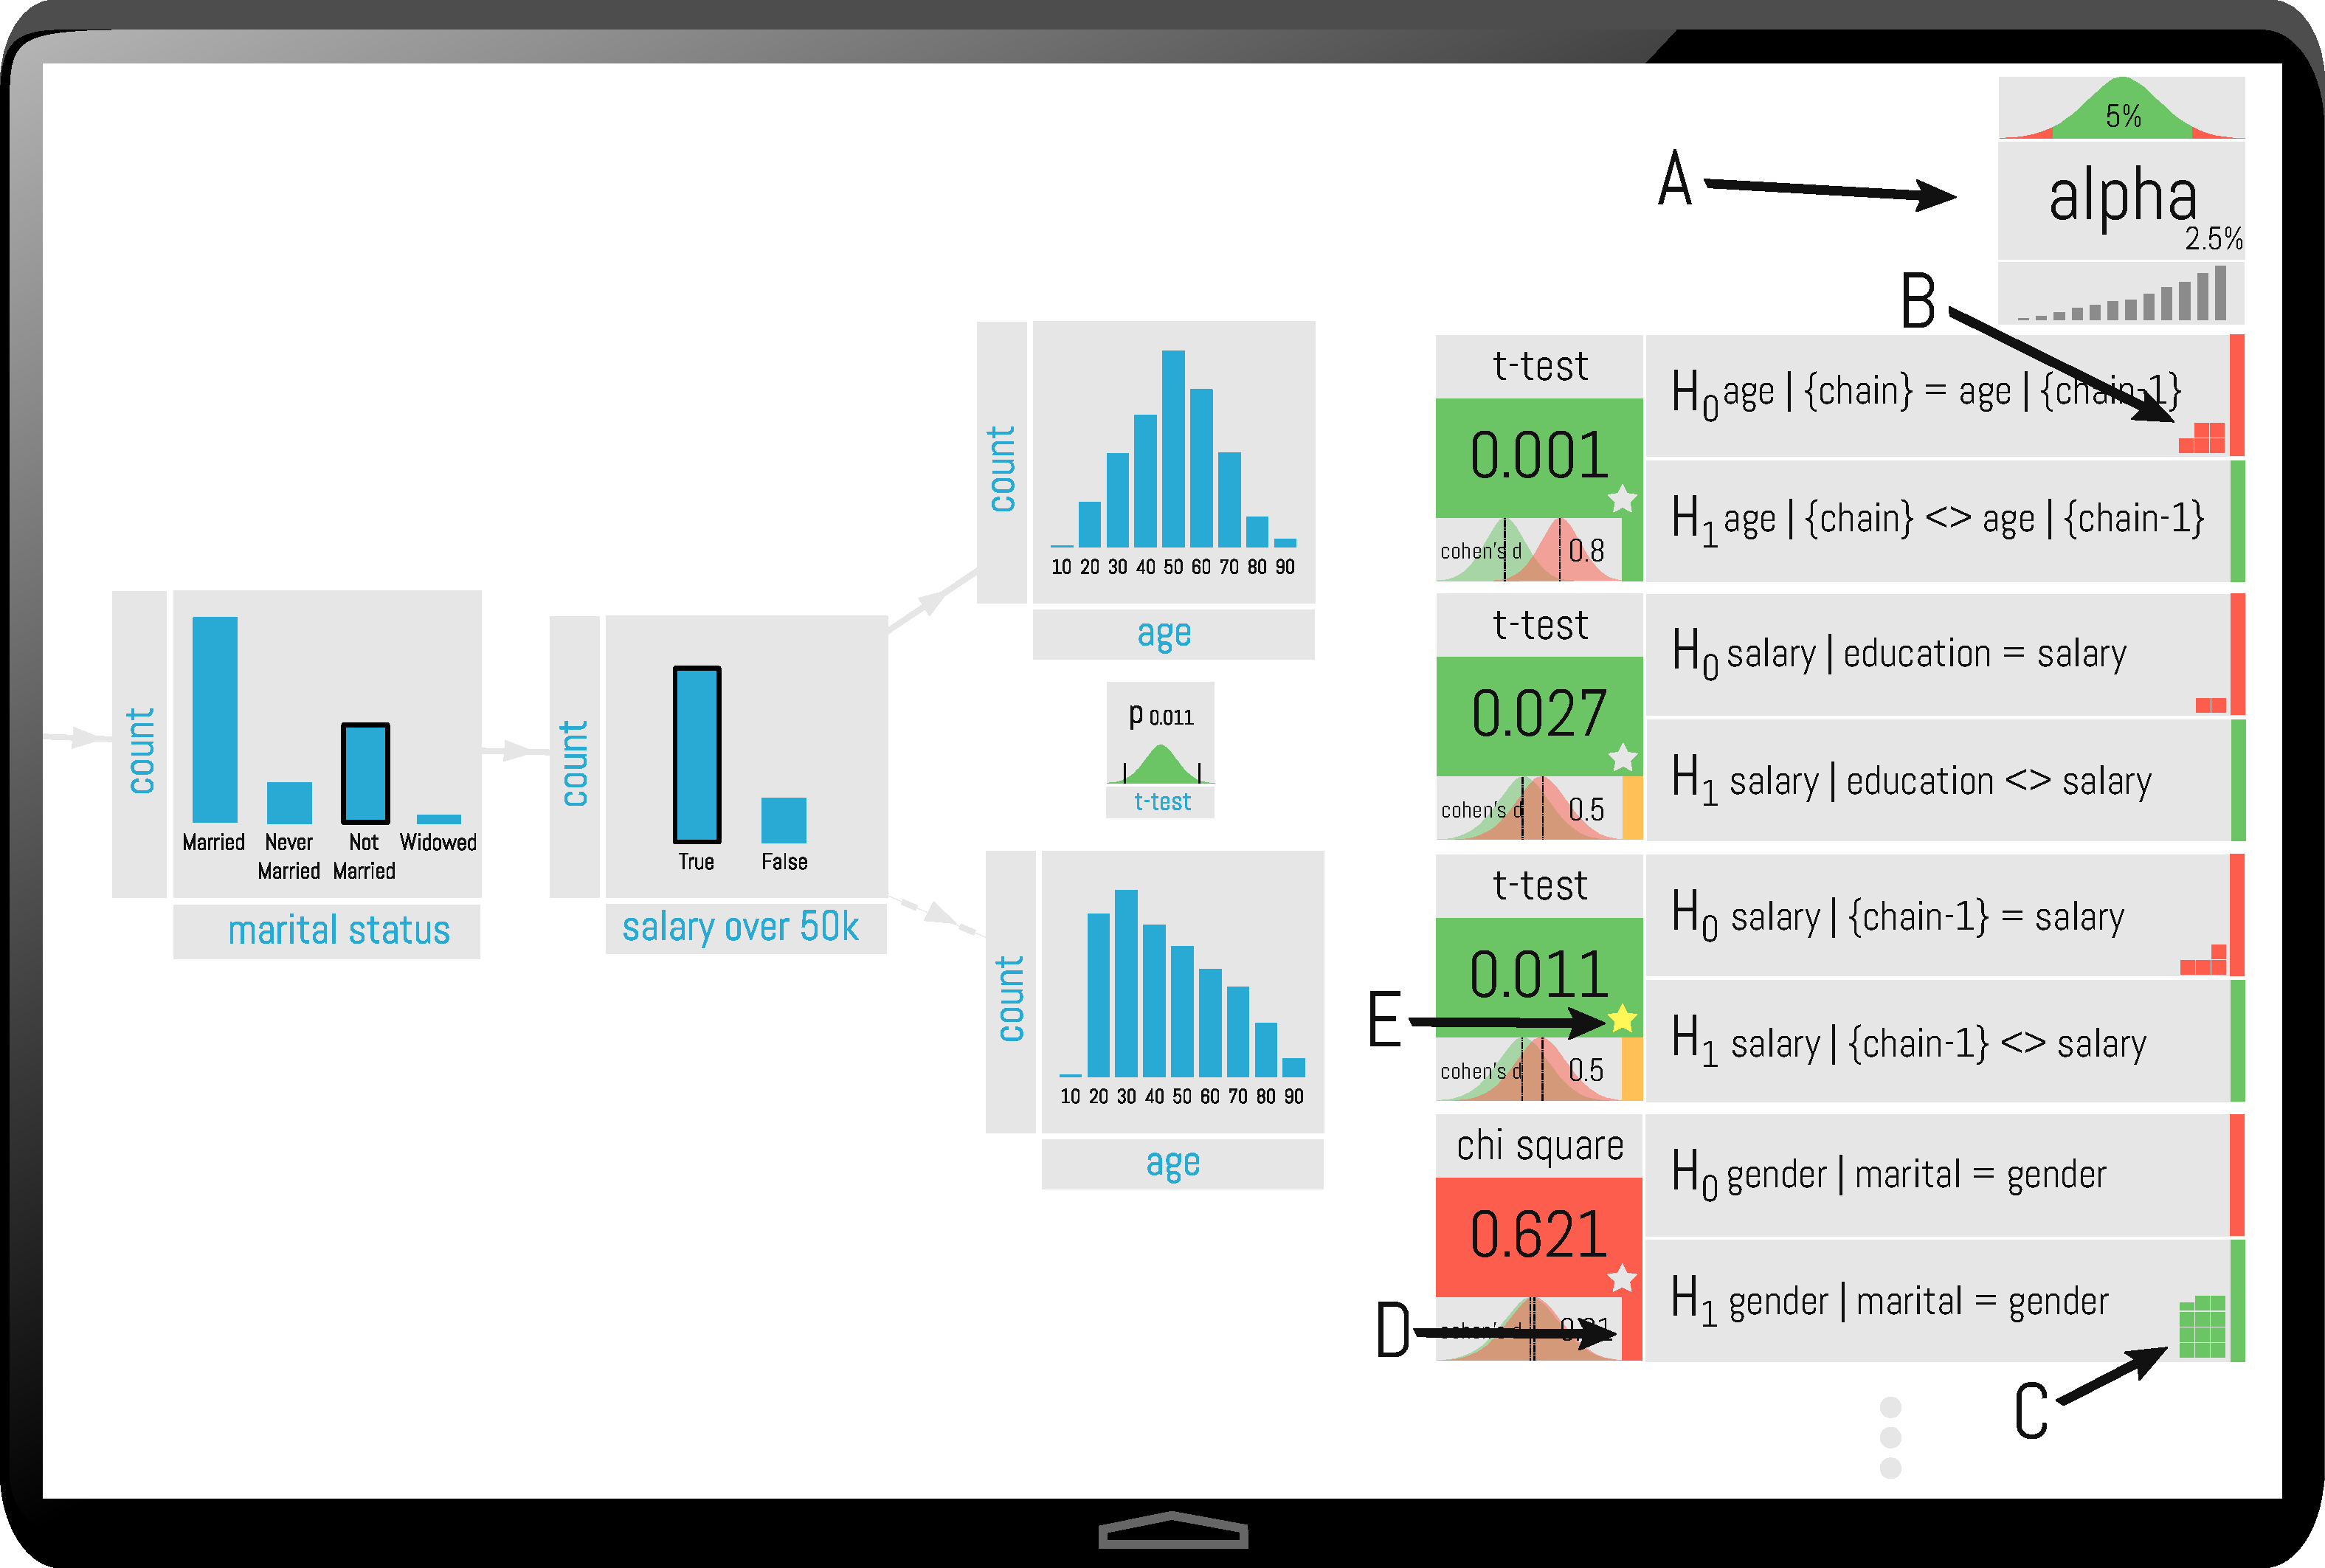
\includegraphics[width=0.48\textwidth]{figures/risk_controller}
\caption{The \system{} User Interface}
\label{fig:riskcontroller}	
\end{figure}

Figure \ref{fig:riskcontroller}	shows the current interface design of \system{} with a risk controller, which incorporates the above ideas, running on a tablet. 
The user interface features an unbounded 2D canvas where chains of visualizations (such as the one shown in Figure \ref{fig:sb}) can be laid out in a free form fashion. 
A ``risk-gauge'' on the right-hand side of the display (Figure \ref{fig:riskcontroller} (A)) serves two purposes: 
%\tim{maybe use a different color for A, B, C in the figure to better highlight them. First I thought A is part of the gauge}
it gives users a summary of the underlying procedure (e.g., the budget for the false discovery rate set to 5\% with current remaining wealth of 2.5\%; %distribution of the \pvals of all tests as 
both explained in the next two sections) and it provides access to a scrollable list of all the hypothesis tests (implicit and explicit) that have been execute so far. 
Each list entry displays details about one test and its results.
Textual labels describe the null- and alternative-hypothesis and color coded \pvals  indicate if the null-hypothesis was rejected or accepted (green for rejected, red for accepted).  
Furthermore, it visualizes the distribution of null-hypothesis and alternative hypothesis and shows its difference, included an indication of its color coded effect size (D). 
%\tim{emanuel, would be good to have a pointer in the figure}
Tap gestures on a specific item allow users to change things like the default hypothesis or the type of test.  
Additionally other information such as an estimation of the size of an additional data  $n^{H1}$ that could make the observation significant can be displayed in each item. 
In the example this information is encoded through a set of small squares (B, C) where each square indicates the amount of data that is in the corresponding distribution. In (B) the five red squares tells us that we need 5x the amount of data from the null-distribution to flip this test form rejected to accepted or conversely in (C) 11.5x the amount of data from the alternative-distribution to rejected this hypothesis. 
Finally, we allow to mark important hypotheses by tapping the ``star'' icons (E). 
%\tim{Again a pointer would be good. }



%\subsection{Overall Control}
%\label{sec:ui:overall}

%- FDR slider
%- Current Realization

%\subsection{The Default Hypothesis}
%\label{sec:ui:default}



%\subsection{Changing The Default Test}
%\label{sec:ui:change}


%\subsection{Additional Information}
%\label{sec:ui:additional}
%- How much more data we need to change the \pval
%- How much more data from the null-hypothesis do we need to add to flip it again



\section{System Design}
\label{sec:system}
\sam{todo: describe system design choices, such as how to generate null hypotheses given user interactions, how to progressively compute marginalized false discovery rate in parallel, etc.}

\section{Conclusion and Future Work}
\label{sec:concl}

In this paper we presented the first automatic approach to controlling the multiple hypothesis  problem during data exploration. 
We showed how the \system{} systems integrates user feedback and presented several multiple hypothesis control techniques based on $\alpha$-investing, which control \emph{mFDR}, and are especially suited for controlling the error for interactive data exploration sessions. 
Finally, our evaluation showed that the techniques are indeed capable of controlling the number of false discoveries using synthetic and real world datasets. 
However, a lot of work remains to be done from  creating and evaluating other types of default hypothesis over developing new testing procedures (e.g., for interactive Bayesian tests) to investigating techniques to recover from cases where the user runs out of wealth. 
Yet, we consider this work as an important first step towards more sustainable discoveries in a time where more data is analyzed than ever before. 




%\section{Acknowledgments}
%This research is funded in part by the Intel Science and Technology Center for Big Data, the NSF CAREER Award IIS-1453171, the Air Force YIP AWARD FA9550-15-1-0144, NSF IIS-1514491, and gifts from SAP, Oracle, Google, Mellanox, and Amazon.

%\clearpage
\balance
\begin{scriptsize}
\bibliographystyle{abbrv}
\bibliography{bib}
\end{scriptsize}

\end{document}